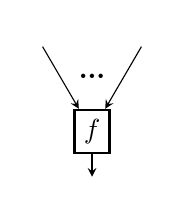
\begin{tikzpicture}[node distance={7mm}, main/.style = {draw, thick}]
\node (X) {$$};
\node (hidden) [right of=X, yshift=-5mm] {\textbf{...}};
\node (Y) [right of=hidden, yshift=5mm] {$$};
\node[main] (task) [below of=hidden] {$f$};
\node (Z) [below of=task] {$$};

\draw[->, >=stealth] (X) -- (task);
\draw[->, >=stealth] (Y) -- (task);
\draw[->, >=stealth] (task) -- (Z);

\end{tikzpicture}
